\documentclass[13pt,a4paper]{article}

\usepackage[utf8]{inputenc}
\usepackage[russian]{babel}
\usepackage[OT1]{fontenc}
\usepackage{amsmath}
\usepackage{amsfonts}
\usepackage{amssymb}
\usepackage{graphicx}

\usepackage{mathtext}

\usepackage{tikz}
\usepackage{pgfplots}
\usepackage[export]{adjustbox}

\usepackage[left=2cm,right=2cm,top=2cm,bottom=2cm]{geometry}
\usepackage{calc}
\usepackage{wrapfig}
\usepackage{setspace}
\usepackage{indentfirst}
\usepackage{subfigure}


\title{
1.4.1.

Изучение физического маятника
}

\author{Семёнов Андрей Б02-016}
\date{11 марта 2021г.}
\begin{document}

\maketitle
\newpage

\textbf{Цель работы:} исследовать зависимость периода колебаний физического маятника от его момента инерции.


\textbf{В работе используются:} физический маятник (однородный стальной стержень), опорная призма, математический маятник, счетчик числа колебаний, линейка, секундомер.

\section{Теоретические сведения}
Физическим маятником называют любое твердое тело, которое под действием силы тяжести может свободно качаться вокруг неподвижной горизонтальной оси. Движение маятника описывается уравнением:

\begin{equation}
	I\frac{d^2\varphi}{dt^2}=M,
	\label{eq:force_moment}
\end{equation}
где $I$$-$момент инерции маятника, $\varphi$$-$угол отклонения маятника от положения равновесия, $t$$-$время, $M$$-$момент сил, действующих на маятник.\\
\begin{wrapfigure}{r}{0.5\textwidth}
   		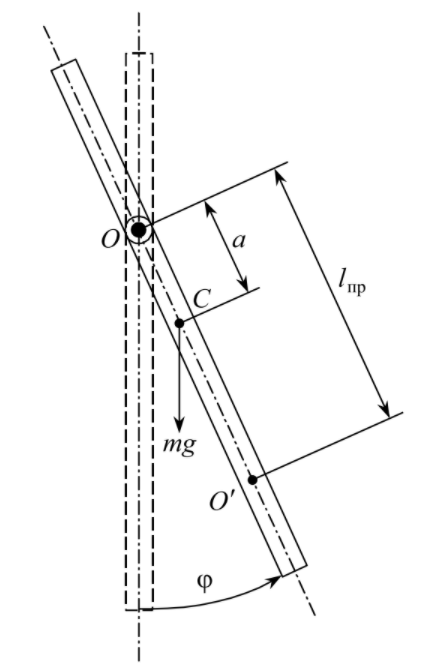
\includegraphics[width=0.4\textwidth]{physpend}
    	\caption{Физический маятник}
    	\label{ris:physpend}
\end{wrapfigure}
В нашей работе в качестве физического маятника \ref{ris:physpend} используется однородный стальной стержень длинны $l$. На стержне закрепляется опорная призма, острое ребро которой является осью качания маятника. Призму можно перемещать вдоль стержня, меняя таким образом расстояние OC от точки опоры маятника до его центра масс. Пусть это расстояние равно $a$, тогда по теореме Гюйгенса-Штейнера:
\begin{equation}
	I=\frac{ml^2}{12}+ma^2,
	\label{eq:inertia_moment}
\end{equation}
Момент силы тяжести равен $M=-mga\sin\varphi$, учтя малость угла $\varphi$ и подставляя это вместе с (\ref{eq:inertia_moment}) в (\ref{eq:force_moment}) получим:
\begin{equation}
	\varphi''+\omega^2\varphi=0,
	\label{eq:osc}
\end{equation}
где 
\begin{equation}
	\omega^2=\frac{ga}{a^2+\frac{l^2}{12}}.
	\label{eq:osc_omega}
\end{equation}
Решением этого уравнение является
\begin{equation}
	\varphi(t)=A\sin(\omega t+\alpha).
	\label{eq:osc_main}
\end{equation}
Амплитуда $A$ и начальная фаза $\alpha$ определяются только только начальными условиями.\\
Период колебаний равен:
\begin{equation}
	T=\frac{2\pi}{\omega}=2\pi\sqrt{\frac{a^2+\frac{l^2}{12}}{ag}}.
	\label{eq:phys_period}
\end{equation}
Видим, что период малых колебаний не зависит ни от фазы, ни от амплитуды колебаний. Изохронность справедлива для всех колебаний, подчиняющихся уравнению (\ref{eq:osc}).\\
Период колебаний математического маятника определяется:
\begin{equation}
	T'=2\pi\sqrt{\frac{l'}{g}}.
	\label{eq:math_period}
\end{equation}
$l'$$-$длина математического маятника. Поэтому величину $l_{pr}=a+\frac{l^2}{12a}$ называют приведённой длиной физического маятника. Точка $O'$ называется центром качания. При качании маятника относительно точки $O'$ егопериод будет таким же, как и при качании относительно точки $O$.  
\begin{wrapfigure}{r}{0.5\textwidth}
   		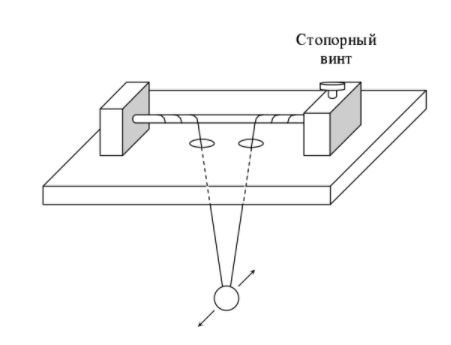
\includegraphics[width=0.4\textwidth]{mathpend}
    	\caption{Математический маятник}
    	\label{ris:mathpend}
\end{wrapfigure}
\newpage
Эти методом можно проверять теоретические сведения. Ещё один метод заключается в проверке правильности формулы (\ref{eq:phys_period}). Входящую в формулу величину $a$ можно изменять, передвигая опорную призму по стержню. В данной работе в качестве математического маятника используется свинцовый шарик, подвешенный на двух расходящихся нитях, как показано на \ref{ris:mathpend}. Длину нитей можно изменять, наматывая их на ось.
\newpage


\section{Выполнение работы}

Имеем утановку со следующими характеристиками:\\
$l=100\pm0,5$см.\\
$m=952,8$г$-$масса стержня


\subsection{Диапазон амплитуд}

Определим диапазон амплитуд, в пределах которого Т не зависит от амплитуды:

\begin{center}
\begin{tabular}{|c|c|c|c|}
\hline
XX & $\varphi$ & $\varphi/2$ & $\varphi/4$ \\ \hline
$t_{100}$, с & 157,4 & 156,38 & 155 \\
\hline
\end{tabular}
\end{center}


\subsection{График $T^2a(a^2)$}
Перемещая опорную призму вдоль стержня, исследуем зависимость периода колебаний T от расстояния а между точкой опоры и центром масс.\\
$\Delta a=0,2$см, тогда:\\
\begin{displaymath}
\Delta(a^2)=\sqrt{2}a\Delta a
\end{displaymath}

\begin{displaymath}
\Delta(T)=\frac{\Delta T}{n}
\end{displaymath}

\begin{displaymath}
\Delta(aT)=aT^2\sqrt{2(\frac{\Delta T}{T})^2 + (\frac{\Delta a}{a})^2}
\end{displaymath}


\begin{table}[h!]
\begin{center}
\begin{tabular}{|c|c|c|c|c|c|c|c|c|c|c|c|c|c|c|c|}
\hline
$a$, см & 3 & 5 & 7 & 9 & 11 & 13 & 17 & 19 & 21 & 23 & 27 & 29 &31 & 33 & 35 \\  \hline
$a^2$, смЕ2 & 9 & 25 & 49 &81 & 121 & 169 & 289 & 361 & 441 & 529 & 729 & 841 & 961 & 1089 & 1225 \\ \hline
$\Delta(a^2)$, смЕ2 & 0,8 & 1,4 & 2 & 2,5 & 3,1 & 3,7 & 4,8 & 5,4 & 5,9 & 6,5 & 7,6 & 8,2 & 8,8 & 9,3 & 9,9 \\ \hline
$T$, с & 1,6 & 1,6 & 1,62 & 1,57 & 1,558 & 1,547 & 1,53 & 1,53 & 1,53 & 1,527 & 1,55 & 1,565 & 1,596 & 1,636 & 1,692 \\ \hline
$\Delta(T)$, с & 0,02 & 0,01 & 0,01 & 0,007 & 0,007 & 0,007 & 0,007 & 0,007 & 0,007 & 0,007 &0,007&0,007&0,007&0,007& 0,007 \\ \hline
$T^2a$, см сЕ2 &7,68&12,8&18,371&22,184&26,701&31,112&39,795&44,477&49,159&53,630&64,868&71,028&78,963&88,324&100,2 \\ \hline
$\Delta(T^2a)$, см сЕ2 &3,5&1,8&1,2&0,9&0,8&0,7&0,7&0,6&0,6&0,6&0,6&0,6&0,6&0,6&0,6 \\ \hline
\end{tabular}
\caption{Результаты измерений и погрешности}
\label{tab:main}
\end{center}
\end{table}

Теперь можем построить график зависимости $T^2a(a^2)$:

\begin{minipage}[h]{2\textwidth}

\begin{tikzpicture}[scale = 1.5]
\begin{axis}[
axis lines = left,
xlabel = {$a^2$, смЕ2},
ylabel = {$T^2a$, см сЕ2},
xmin = 0, xmax = 1300,
ymin = 0, ymax = 110,
ymajorgrids = true,
xmajorgrids = true
]
\addplot[
mark = square, 
mark options = {
scale = 1.5, 
fill = black,
},
ymajorgrids = true,
xmajorgrids = true,
color = black
] coordinates {
(9, 7.68) (25, 12.8) (49, 18.371) (81, 22.184) (121, 26.701) (169, 31.112) (289, 39.795) (361, 44.477) (441, 49.159) (529, 53.630) (729, 64.868) (841, 71.028) (961, 78.963) (1089, 88.324) (1225, 100.2)
}; 
%\addplot [
domain=0:100, 
samples=1000, 
color=red,
]
{6.563+x*0.129};
\end{axis}
\end{tikzpicture}
\end{minipage}


\begin{figure}[h!]
\begin{center}
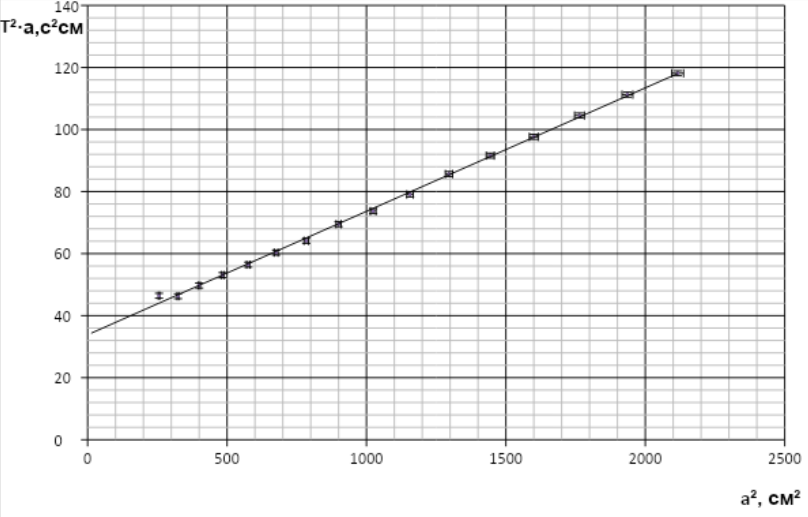
\includegraphics[width=\textwidth]{grafik}
\caption{График}
\label{ris:grafik}
\end{center}
\end{figure}


\subsection{Находим $g/4\pi^2$ и $l^2/12$}

\begin{displaymath}
T=2\pi\sqrt{\frac{a^2 + \frac{l^2}{12}}{ag}}
\end{displaymath}

\begin{displaymath}
T^2=\frac{4\pi^2a}{g}+\frac{4\pi^2l^2}{12ag}
\end{displaymath}

\begin{displaymath}
T^2a=\frac{4\pi^2}{g}a^2+\frac{4\pi^2l^2}{12g}
\end{displaymath}


$y=kx+b$, где $k=\frac{4\pi^2}{g}=(0,0398\pm0,0004); s^2cm^{-1}\Rightarrow \frac{g}{4\pi^2}=(0,251\pm0,002);\frac{m}{s^2}$
Соответсвенно получаем:\\
$g=(9,87\pm0,08)$ $\frac{m}{s^2}$

\begin{displaymath}
b=\frac{4\pi^2l^2}{12g}=(0,338\pm0,003); s^2m
\end{displaymath}
$\frac{l^2}{12}=(0,085\pm0,002)$мЕ2
Отсюда сразу получаем экспериментально значение длинны стержня:
$l=(1,02+0,01)$м


\subsection{Немного математического маятника}

Подберём длину математического маятника так, чтобы в пределах точности измерений периоды колебаний обоих маятников совпали.
Согласно теоретическим вычислениям:\\
$l_{pr}=58,8$см

Экспериментальное же значение:\\
$l_{pr exp}=(59\pm0,2)$см

Данные величины соыпадают в пределах погрешности 


\subsection{Обратимость точки подвеса(опоры) и центра качания физического маятника}

Проверим на опыте обратимость точки подвеса и центра качения физического маятника(то есть при качании маятника вокруг $O'$ период будет таким же, как и при качании вокруг $O$).

При $а=(20\pm0,2)$см   $Т_{а}=(1,58\pm0,2)$с  ,  $a'= l_{pr} – а= l_{m}-а=(42\pm0,2)$см 
При $a’$   $Т_{a’}=(1,57\pm0,2)$с

С учетом погрешности их периоды совпадают.

\section{Выводы}
\begin{enumerate}
\item Мы получили довольно точные значения $g$ и $l$.
\item Подтвердили обратимость точки подвеса (опоры) и центра качания физического маятника.
\item Построили график зависимости $T^2a(a^2)$.
\end{enumerate}


\section{Контрольные вопросы}

\textbf{1. При каких упрощающих предположениях была выведена формула (\ref{eq:phys_period})?}\\
\\
Формула получается при малости угла отклонения тела от положения равновесия, когда допустимо приближение $\sin\varphi\approx\varphi$.\\
\textbf{2. При каком расстоянии от центра масс до точки подвеса период колебаний маятника минимален?}\\
\\
Период колебаний будет минимальным при расстоянии $\frac{2}{2\sqrt{3}}$, которое можно вычислить приравняв $\frac{dT^2}{da}$  к нулю. При очень больших или очень малых a период стремится к бесконечности, а значит в точке, где производная ноль находится минимум графика $T^2(a)$ , и он равен $T=2\pi\sqrt{sqrt{3}\frac{l}{g}}$.\\
\\
\textbf{3. Как будет вести себя физический маятник, если совместить точку его подвеса с центром масс?}\\
\\
При смещении точки подвеса в точку центра масс, стержень не будет колебаться, а будет оставаться в том положении, в котором его оставить, ведь момент силы тяжести будет равен 0.\\
\\
\textbf{4. С какой целью в данной работе математический маятник подвешивается на двух нитях?}\\
\\
4.	Математический маятник подвешивается на 2 нитях для того, чтобы исключить колебания во всех направлениях, кроме изучаемого.\\
\\
\textbf{5. Сформулируйте и докажите теорему Гюйгенса-Штейнера.}\\
\\

\begin{figure}[h!]
	\begin{center}
		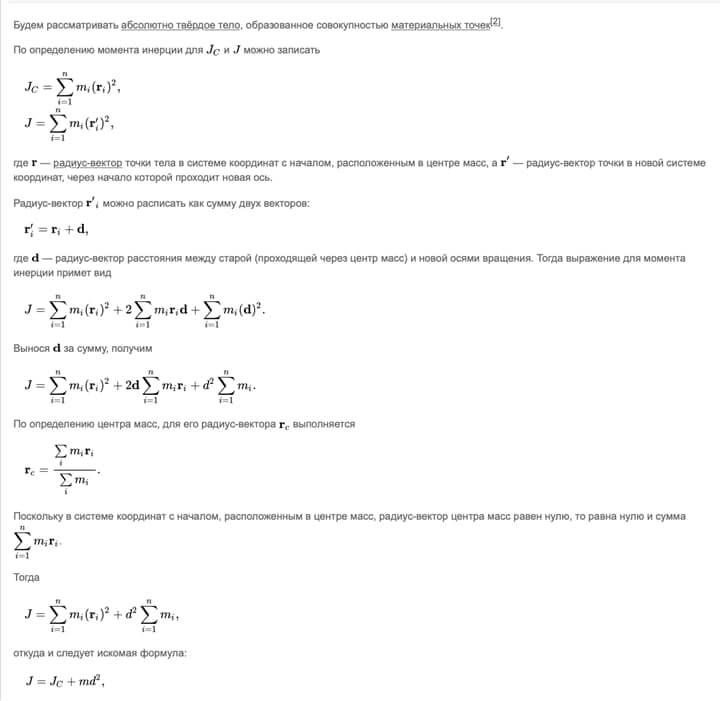
\includegraphics[width = 1.3\textwidth]{theorem}
		\label{fig:theorem}
	\end{center}
\end{figure}

\end{document} 